\section{Domain Modelling}
\subsection{Couse Navigation}
\begin{figure}[ht]
    \centering
    \begin{minipage}{0.3\textwidth}
        \centering
        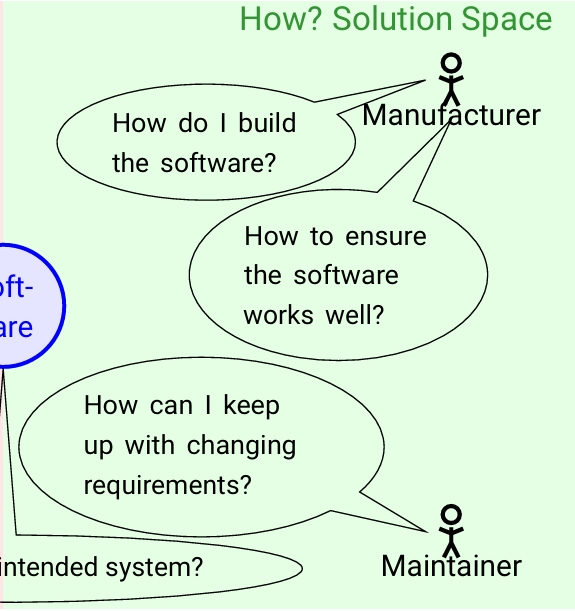
\includegraphics[width=\textwidth]{Images/Course Navigation 1.jpeg}
    \end{minipage}
    \hfill
    \begin{minipage}{0.3\textwidth}
        \centering
        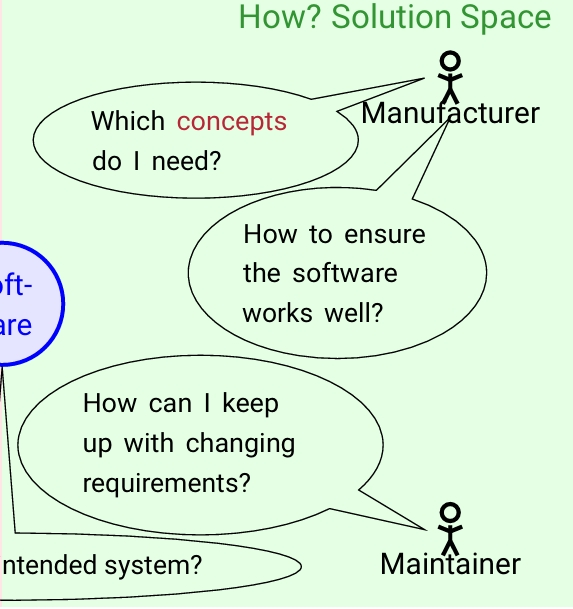
\includegraphics[width=\textwidth]{Images/Course Navigation 2.jpeg}
    \end{minipage}
    \hfill
    \begin{minipage}{0.3\textwidth}
        \centering
        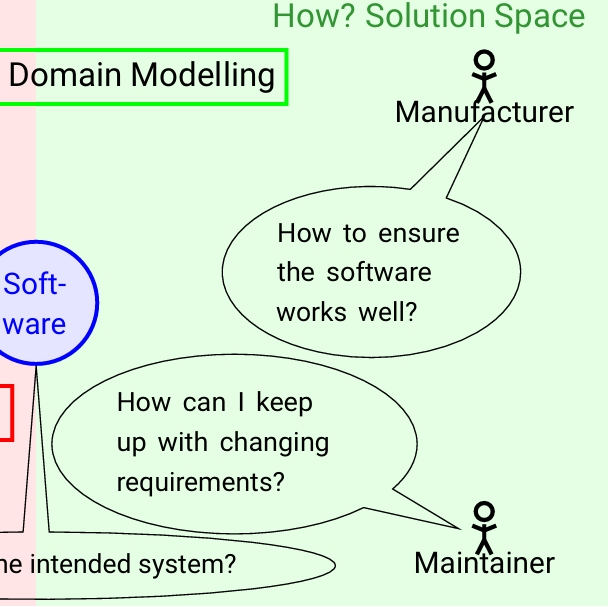
\includegraphics[width=\textwidth]{Images/Course Navigation 3.jpeg}
    \end{minipage}
\end{figure}

\subsection{General Approach: Object-oriented Analysis \& Design}
\begin{defBox}
    In the solution space we use \red{Object-oriented Analysis \& Design} (OOAD)
\end{defBox}
\begin{defBox}[title=Motivation]
    \begin{itemize}
        \item Considered \red{state-of-art}
        \item \red{Widely-used} in industrial practice, many software processes
        \item Numerous \red{training} resources available
        \item Compatible with wide-spread visual modeling notation \red{UML}
        \item Compatible with \red{C++, C\#, JAVA, KOTLIN, SCALA, ...}
    \end{itemize}
\end{defBox}

\subsection{Domain Modelling}
\begin{defBox}[title=Domain Modelling]
    Fixing the \blue{terminology} and \blue{fundamental activities} of the \red{solution space}
    \begin{itemize}
        \item \red{Why:} Helps to identify the \red{relevant} concepts and tasks of a domain
        \item \red{Prerequisite:} \red{Requirements analysis} and \red{use case analysis} are done
        \item \red{Context:} Part of \red{object-oriented analysis} (OOA)
        \item \red{Heuristics:} Only performed for the \red{tasks at hand}
    \end{itemize}
\end{defBox}
\blue{Curtis'law}: \enquote{... good designs require deep application knowledge.}
\begin{defBox}
    Domain model must be \red{validated with \blue{Client}}
\end{defBox}
\begin{infoBox}
    \fatsf{Domain Modeling} beschreibt den Prozess, die Fachterminologie und grundlegende Aktivitäten eines bestimmten Problembereichs (der Domäne) festzulegen und zu strukturieren. Es dient dazu, die relevanten Konzepte und Aufgaben einer Domäne zu indentifizieren und damit die Grundlage für eine lösungsorientierte Systementwicklung zu schaffen.
\end{infoBox}

\begin{infoBox}[title=Warum Domain Modeling?]
    \begin{itemize}
        \item \fatsf{Ziel:} Domain Modeling hilft, die relevanten Konzepte und Aufgaben zu erkennen, die zur Lösung der Anforderungen eines bestimmten Problembereichs nötig sind. Es stellt sicher, dass alle wichtigen Elemente und Interaktionen einer Domäne klar definiert und verstanden sind.
        \item \fatsf{Voraussetzung:} Um ein Domain Model zu erstellen, sollten die \fatsf{Anforderungen} bereits erfasst und durch \fatsf{Use Cases analysiert} worden sein. Das Domain Model baut darauf auf, indem es Konzepte aus diesen Anforderungen abbildet.
    \end{itemize}
\end{infoBox}

\begin{infoBox}[title=Kontext und Ziele des objektorientierten Domain Modeling]
    \begin{itemize}
        \item \fatsf{Teil der Objektorientierten Analyse (OOA):} Somain Modeling ist eng mit der objektorientierten Analyse verbunden und bildet einen Schritt in der objektorientierten Softwareentwicklung.
        \item \fatsf{Curtis'Gesetz:} Ein tiefes Verständnis der Domäne ist notwendig, um gute Entwürfe zu erstellen. Es erfordert daher, dass Entwickler und Fachleute, die das Modell erstellen, die Domäne gut verstehen, um ein realistisches Modell zu entwickeln.
        \item \fatsf{Validierung:} Das Domain Model muss von den Auftraggebern oder Fachexperten validiert werden, um sicherzustellen, dass die erfassten Konzepte korrekt und vollständig sind.
    \end{itemize}
\end{infoBox}
\begin{defBox}[title=Goal of an Object-Oriented Domain Model]
    Decompose the domain into \red{concepts} or \red{objects} that represent the \red{real world} (as captured in the requirements specification)
\end{defBox}
\begin{infoBox}[title=Ziel eines Objektorientierten Domain Models]
    \begin{itemize}
        \item Das Ziel besteht darin, die Domäne in \fatsf{Konzepte oder Objekte} zu unterteilen, die die reale Welt repräsentieren, wie sie in der Anforderungsanalyse dokumentiert wurden.
        \item Dies bildet die Basis für das spätere \fatsf{Softwaredesign}, in dem diese Konzepte als Objekte oder Klassen im Code umgesetzt werden.
    \end{itemize}
\end{infoBox}
\begin{defBox}[title=How to create an Object-Oriented Domain Model]
    \begin{itemize}
        \item Identify the set of \blue{conceptual} \red{classes} and fundamental \red{actions}
    \end{itemize}
    \red{Iteratively} completed and forms the basis for the \red{software design}
\end{defBox}
\begin{infoBox}[title=Erstellung eines objektorientierten Domain Models]
    \begin{itemize}
        \item Die grundlegenden Aktivitäten umfassen das Identifizieren und Definieren der \fatsf{konzeptuellen Klassen} (z.B. Objekte und Entitäten) und \fatsf{fundamentalen Aktionen} (Methoden und Interaktionen), die für die Domäne relevant sind.
        \item Dieser Prozess wird in der Regel iterativ durchgeführt, da das Modell schrittweise vervollständigt und verfeinert wird.
    \end{itemize}
\end{infoBox}
\begin{defBox}[title=Synonyms for Domain Model]
    \begin{itemize}
        \item Conceptual model, domain object model, analysis object model \enquote{\red{Konzeptmodell}}, \enquote{\red{Analysemodell}}
    \end{itemize}
\end{defBox}

\subsection{Conceptual Classes}
\begin{defBox}[title=Conceputal class \enquote{Konzeptklasse}]
    \red{Conceptual classes} represent ideas, things or objects in the domain.\\
    A conceptual class has
    \begin{itemize}
        \item a \red{name} or symbol representing the class,
        \item an \red{intention} (\endquote\red{Bedeutung}),
        \item an \red{extension} (\enquote{\red{Ausprägung}}, \enquote{\red{Extension}}).
    \end{itemize}
    The \red{extansion} \blue{contains} the domain elements the conceptual class represents.
\end{defBox}
\begin{defBox}
    Domain concepts/conceptual classes are \red{not} software objects - They drive from the \red{problem space}
\end{defBox}

\section{UML Class Diagrams}
\subsection{Visualization of Domain Models}
Domain models are visualized using \red{UML class diagrams}\\
\blue{But} with suitable restrictions to emphasize \red{domain} modelling:
\begin{itemize}
    \item Only domain \red{objects} and conceptual \red{classes}
    \item Only \red{associations}, no aggregation, no composition
    \item Classes may have \red{attributes} (used sparingly), but \red{no operations}
\end{itemize}
\begin{defBox}
    UML class diagram of domain model is called \red{conceptual perspective model} \enquote{Modell der Konzeptperspektive}
\end{defBox}
\begin{figure}[h]
    \centering
    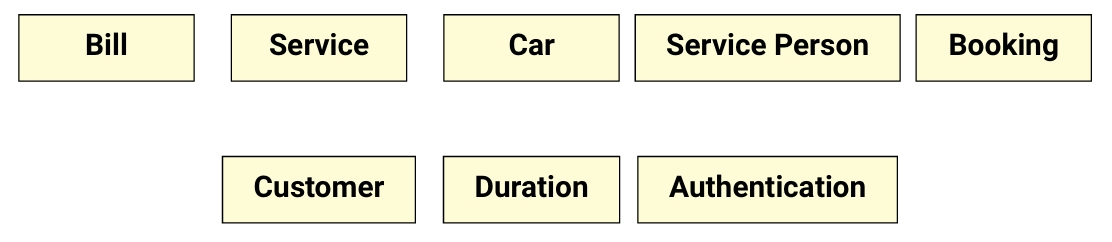
\includegraphics[width=1\textwidth]{Images/CaSh Booking System.jpeg}
\end{figure}
\begin{itemize}
    \item \red{Bookings} are made by \red{customers}
    \item Customers must have \red{authentication} to make a booking
    \item Each booking is for exactly one \red{car}
    \item The monthly \red{bill} comprises all completed and unpaid bookings
    \item Each booking is for a \red{duration} of between 30 minutes and four weeks
    \item A customer connot have more than three active bookings
    \item Each car needs to have a regular \red{service} carried out by a \red{service person}
\end{itemize}
\begin{defBox}[title=Classes]
    A (conceptual) \red{class} describes a set of (domain) objects\\
    An object is an individual thing with a \red{state} and \red{relations} to other objects
\end{defBox}
\subsection{Properties of Conceptual Classes:}
\subsubsection*{Attributes}
\begin{figure}[h]
    \centering
    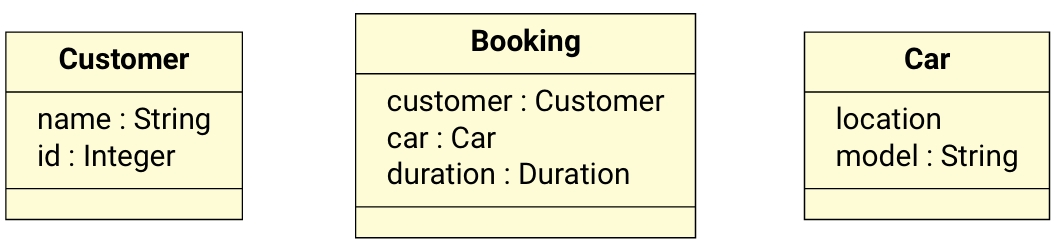
\includegraphics[width=1\textwidth]{Images/Attributes.jpeg}
\end{figure}
\begin{itemize}
    \item Logical data values of an object (class instance, domain element)
    \item Map objects of the containing class to objects of their target type
\end{itemize}
\begin{infoBox}[title=Was sind Attribute?]
    \begin{itemize}
        \item \fatsf{Attribute} sind logische Datenwerte, die eine Klasse und deren Instanzen (also Objekte) näher beschreiben. Sie entsprechen den Informationen, die eine Klasse im System speichert.
        \item Sie stellen eine Abbildung von Objekten der Klasse auf ihre Zielwerte dar. Beispielsweise könnte eine Klasse \fatsf{Person} das Attribut \fatsf{Name} haben, welches Objekte der Klasse \fatsf{Person} auf konkrete Namenswerte (z.B. \enquote{Alice}) abbildet.
    \end{itemize}
\end{infoBox}
During \red{domain modelling:}
\begin{itemize}
    \item Identify attributes of conceptual classes\\
    needed to satisfy \red{information requirements}
    \item \red{Limit} number of attributes to scope of treated scenarios
\end{itemize}
\begin{infoBox}[title=Attribute während der Domänenmodellierung]
    \begin{enumerate}
        \item \fatsf{Identifizierung der benötigten Attribute:}
        \begin{itemize}
            \item In der Phase der Domänenmodellierung ist es wichtig, Attribute nur dann zu definieren, wenn sie tatsächlich zur Erstellung der Informationsanforderungen relevant sind. Beispielsweise könnte ein Attribut \fatsf{Adresse} für die Klasse \fatsf{Kunde} nur dann notwendig siein, wenn Adressinformationen für die Geschäftprozesse erforderlich sind.
        \end{itemize}
        \item \fatsf{Begrenzung auf szenario-relevante Attribute:}
        \begin{itemize}
            \item Es ist ratsam, die Anzahl der Attribute auf das Wesentlich zu beschränken, um die Modellkomplexität zu verringern. Attribute sollten daher nur die Informationen abdecken, die für die im Modell behandelten Szenarien erforderlich sind.
        \end{itemize}
        \item \fatsf{Begrenzung auf szenario-relevante Attribute:}
        \begin{itemize}
            \item Es ist ratsam, die Anzahl der Attribute auf das Wesentliche zu beschränken, um die Modellkomplexität zu verringern. Attribute sollten daher nur die Informationen abdecken, die für die im Modell behandelten Szenarien erforderlich sind.
        \end{itemize}
    \end{enumerate}
\end{infoBox}
\subsection{UML Model Element Class: Simplified Syntax for Domain Modelling}
\begin{figure}[h]
    \centering
    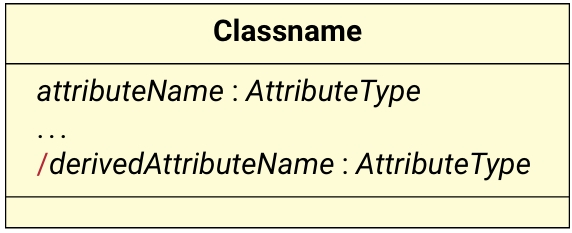
\includegraphics[width=0.5\textwidth]{Images/Class.jpeg}
\end{figure}

\begin{defBox}[title=UML Class Elements and Conventions]
    \begin{itemize}
        \item \red{Class Name:} Class names start always with an upper case letter
        \item \red{Attribute:} \blue{Attribute name:} starts with a lower case letter\\
        \blue{Attribute type:} pre-defined type or other domain model class (type can be \red{omitted} in domain modelling)
        \begin{infoBox}
            In der Phase der Domänenmodellierung ist es nicht zwingend erforderlich, den Typ jedes Attributes anzugeben. Oft genügt es, das Attribut selbst zu identifizieren, um den Zweck des Modells klar darzustellen.
        \end{infoBox}
        \item \red{Derived Attribute:} name prefixed by a slash ('\red{\textbackslash}')\\
        Value computable from existing infomration
    \end{itemize}
\end{defBox}
\begin{infoBox}[title=Abgeleitet Attriubte]
    \begin{itemize}
        \item Ein \fatsf{abgeleitetes Attribut} ist ein Attribut, dessen Wert aus anderen vorhandenen Informationen berechnet werden kann. Solche Attribute werden mit einem Schrägstrich (/) vor dem Namen gekennzeichnet.
        \item \fatsf{Beispiel:} Ein Attribut \fatsf{/Gesamtpreis} in der Klasse \fatsf{Rechnung} könnte als Summe der einzelnen Positionen berechnet werden, anstatt separat gespeichert zu werden.\\
        \fatsf{Notation:} /Gesamtpreis zeigt an, dass dieses Attribut nicht manuell eingegeben wird, sondern als Ergebnis einer Berechnung oder Ableitung verfügbar ist.
    \end{itemize}
\end{infoBox}

\subsection{Example: Derived Attribute}
\begin{figure}[h]
    \centering
    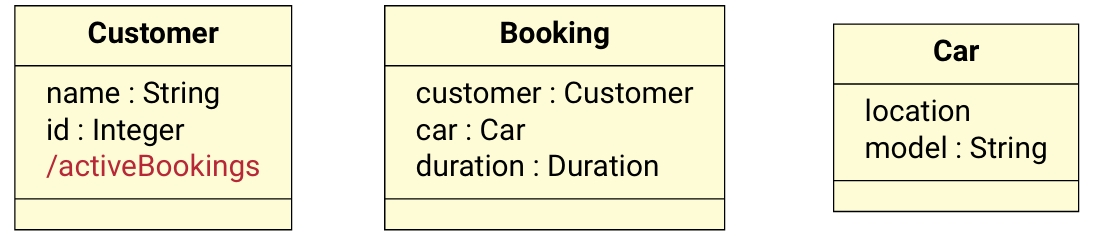
\includegraphics[width=1\textwidth]{Images/Derived Attribute.jpeg}
\end{figure}
\begin{defBox}[title=Example (Active Boodings)]
    \begin{itemize}
        \item The \red{active bookings} of a customer are all not yet completed bookings
    \end{itemize}
    The active bookings for a customer can be computed:\\
    \blue{Collect all bookings of the customer whose end time is not past the current time}\\
    Derived attributes are usually not assigned values independently
\end{defBox}

\subsection{CaSh Booking System: Associations (Relations)}
\begin{figure}[h]
    \centering
    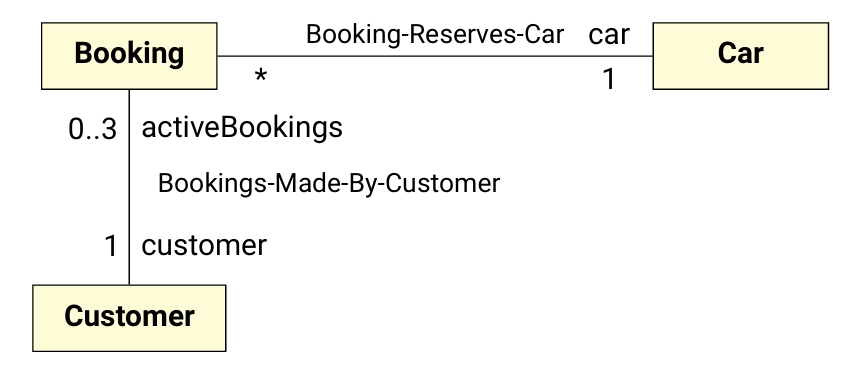
\includegraphics[width=1\textwidth]{Images/Associations (Relations).jpeg}
\end{figure}
\begin{itemize}
    \item \red{Bookings} are made by \red{customers}
    \item A customer cannot have more than \red{three} active bookings
    \item Each booking is for \red{exactly} one car
    \item A car may appear in an arbitrary number of bookings
\end{itemize}

\clearpage
\subsection{Syntax of UML Association}
\begin{figure}[h]
    \centering
    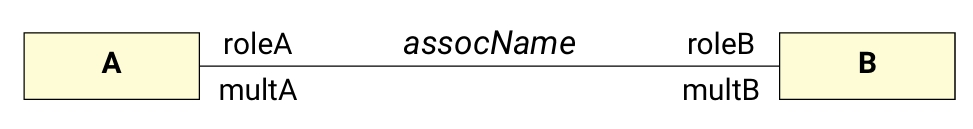
\includegraphics[width=1\textwidth]{Images/Syntax of UML Asociation.jpeg}
\end{figure}
\blue{An} \red{association} \blue{is a relation among classes with the elements:}
\begin{itemize}
    \item Name (optional)
    \item Two association ends called \red{roles}, each with:
    \begin{itemize}
        \item A \red{role name} (defaults to class name starting with lower case letter)
        \item A \red{multiplicity} (defaults to multiplicity 1)\\
        Possible multiplicities: * or a ..b\\
        a, b are \red{value specifications} (numbers expressions); upper bound incl. *
        \item A \red{navigability} (defaults to bi-directional, not used for conceptual classes)
    \end{itemize}
\end{itemize}
\begin{figure}[h]
    \centering
    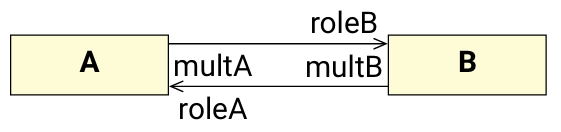
\includegraphics[width=0.5\textwidth]{Images/navigability.jpeg}
\end{figure}

\subsection{Generalizations of Concepts}
\begin{figure}[h]
    \centering
    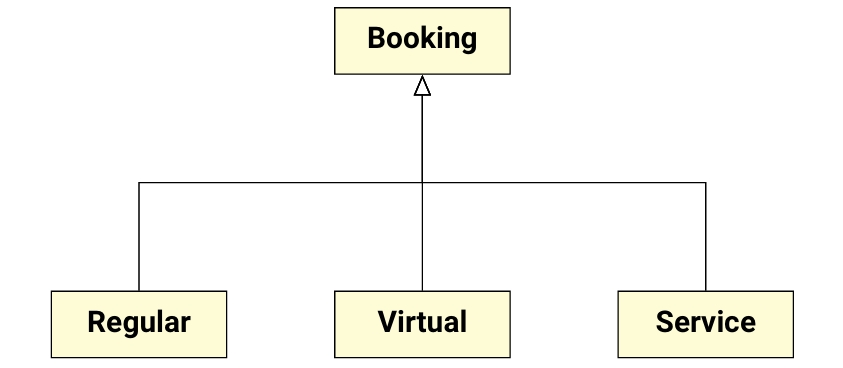
\includegraphics[width=0.5\textwidth]{Images/Generalizations of Concepts.jpeg}
\end{figure}
\begin{itemize}
    \item There are different types of bookings: regular, virtual, service
\end{itemize}

\subsection{Elicitation of Domain Model for a New Domain: Workflow}
\begin{enumerate}
    \item Find the \red{conceptual classes}\\
    Strategies:
    \begin{itemize}
        \item \red{Re-use} or modify an existing model
        \item Use a category \red{list}
        \item Identify \red{noun phrases}
    \end{itemize}
    \item Draw elicited concepts as a classes in a UML class diagram
    \item Add \red{attributes}
    \item Add \red{associations}
\end{enumerate}
\begin{defBox}
    Use the domain vocabulary: The CaSh model should use names like \red{Customer} instead of \blue{Person}
\end{defBox}
\begin{infoBox}
    Die \fatsf{Erhebung (Elicitation) eines Domain Models für eine neue Domäne} ist ein strukturierter Prozess bei dem relevante Konzepte und Beziehungen identifiziert und in ein Modell übertragen werden. Die folgende Übersicht beschreibt die einzelnen Schritte dieses Workflows:
\end{infoBox}
\begin{infoBox}[title=Workflow zur Erstellung eines Domain Models]
    \begin{enumerate}
        \item \fatsf{Konzeptuelle Klassen finden}\\
        Die Konzeptklassen sind die grundlegende Bausteine des Domain Models. Sie repräsentieren wichtige Objekte oder Entitäten in der Domäne, z.B. \enquote{Kunde} oder \enquote{Produkt}. Es gibt mehrere Strategien, um diese Klasse zu identifizieren:
        \begin{itemize}
            \item \fatsf{Vorhandenes Modell wiederverwenden oder anpassen:} Prüfen, ob es bereits ein ähnliches Modell gibt, das an die aktuelle Domäne angepasst werden kann.
            \item \fatsf{Kategorie-Liste verwenden:} Eine Liste typischer Kategorien wie \enquote{Personen}, \enquote{Objekte}, \enquote{Orte} oder \enquote{Transaktionen} kann helfen, wichtige Konzepte zu finden.
            \item \fatsf{Substantivphasen identifizieren:} In den Anforderungen nach Substantiven suchen, die Konzepte darstellen könnten (z.B. \enquote{Kunde}, \enquote{Termin}).
        \end{itemize}
        \item \fatsf{Konzepte als Klassen in einem UML-Klassendiagramm darstellen}
        \begin{itemize}
            \item Die identifizierten Konzeptklassen werden nun in einem \fatsf{UML-Klassendiagramm} als einzelne Klassen mit Namen dargestellt
            \item Dieses Diagramm hilft, die Konzepte zu visualisieren und zeigt, wie sie in Beziehung zueinander stehen könnten.
        \end{itemize}
        \item \fatsf{Attribute hinzufügen}
        \begin{itemize}
            \item In jedem Konzept wird überlegt, welche spezifischen \fatsf{Eigenschaften oder Merkmale (Attribute)} erforderlich sind.
            \item Zum Beispiel könnte die Klasse \enquote{Kunde} Attribute wie \enquote{Kundenname} und \enquote{Kundennummer} haben.
        \end{itemize}
        \item \fatsf{Assoziationen hinzufügen}
        \begin{itemize}
            \item Assoziationen zeigen die \fatsf{Beziehungen zwischen den Klassen}. Diese Beziehungen geben Einblick in die Interaktionen zwischen den Konzepten und wie sie zusammenarbeiten.
            \item Zum Beispiel könnte eine Assoziation zwischen den Klassen \enquote{Kunde} und \enquote{Bestellung} die Beziehung \enquote{Kunde erstellt Bestellung} darstellen.
        \end{itemize}
    \end{enumerate}
\end{infoBox}

\clearpage
\subsection{Re-using an Existing Model}
\begin{figure}[h]
    \centering
    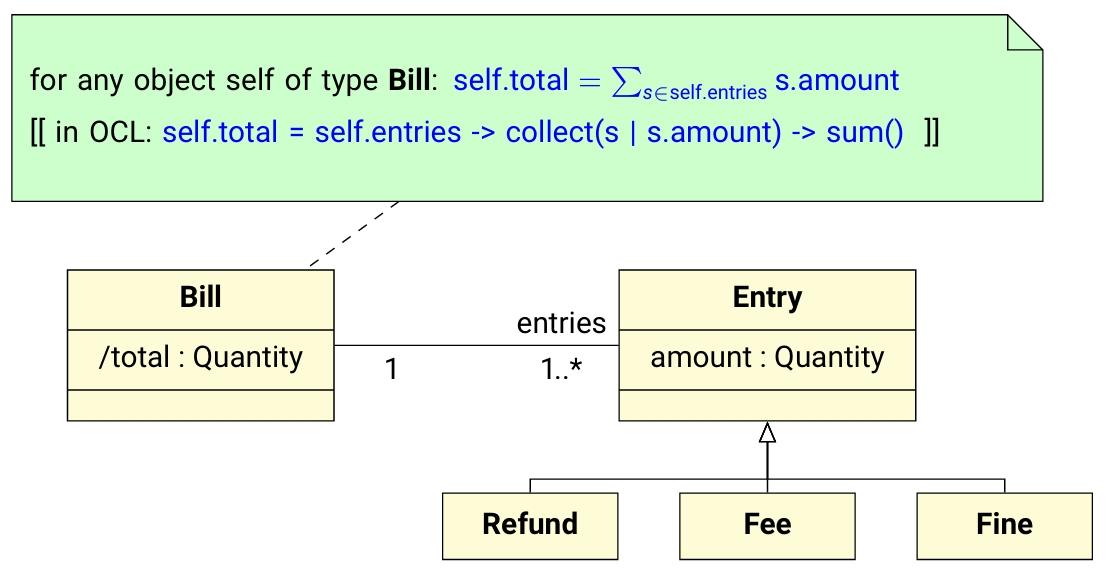
\includegraphics[width=1\textwidth]{Images/Re-using an Existing Model.jpeg}
\end{figure}
\begin{infoBox}[title=UML-Diagramm und Beziehungen]
    Das UML-Diagramm zeigt zwei zentrale Klassen und ihre Attribute:
    \begin{itemize}
        \item \fatsf{Bill:} Repräsentiert eine Rechnung, die das Attribut \textbackslash total hat. Das \textbackslash vor dem Attributnamen weist darauf hin, dass es ein berechnetes Attribut ist.
        \item \fatsf{Entry:} Repräsentiert einen einzelnen Eintrag auf der Rechnung mit dem Attribut \fatsf{amount}, das den Betrag des Eintrags speichert
        \item \fatsf{Assoziationen:}
        \begin{itemize}
            \item \fatsf{eintries:} Eine \enquote{Bill} enthält eine oder mehrere \enquote{Entry}-Objekte (dargestellt durch die Kardinalität \enquote{1..*}). Diese Beziehung zeigt, dass jede Rechnung eine Liste von Einträgen hat, und jeder Eintrag gehört genau zu einer Rechnung.
        \end{itemize}
    \end{itemize}
    Zusätzliche Klassen wie \fatsf{Refund, Fee} und \fatsf{Fine} sind spezialisierte Typen von Entry. Diese Subklassen könnten spezifische Arten von Einträgen darstellen, z.B. \enquote{Erstattung} (Refund), \enquote{Gebühr} (Fee) oder \enquote{Strafe} (Fine).
\end{infoBox}
\subsection{Identification of Concept Classes: List of Conceptual Class Categories}
\begin{defBox}[title=Some Categories]
    \begin{itemize}
        \item Physical or tangible objects
        \item Specifications or description of things
        \item Locations
        \item Events
        \item Transactions
        \item Transaction items
        \item Organizations
        \item Roles (of people, organizations, etc.)
        \item Containers
        \item ...
    \end{itemize}
\end{defBox}
\subsection{Using a Category: Example}
\begin{table}[H]
    \centering
    \rowcolors{2}{\thepagecolor}{fgcolor!10!\thepagecolor}
    \renewcommand{\arraystretch}{1.2}
    \begin{tabular}{lll}
        \toprule
        Conceptual Class Category & Conceptual Classes (in CaSh) \\
        \midrule
        Business transaction & Bill, Payment\\
        Transaction line item & Entry\\
        Product or service related to a transaction or to a transaction line item & Refund, Rent, Fine\\
        Place where transaction is recorded & Registry\\
        Roles of people or organizations related to a transaction (actors in use cases) & Customer, Accountant\\
        Location where transaction executed & Website\\
        Noteworthy events, with a time or place that needs to be remembered & Bill, Booking\\
        \bottomrule
    \end{tabular}
\end{table}
\begin{infoBox}[title=Kategorien konzeptioneller Klassen]
    \begin{enumerate}
        \item \fatsf{Physische oder greifbare Objekte}
        \begin{itemize}
            \item Beziehen sich auf reale, konkrete Objekte.
            \item \fatsf{Beispiele:} Geräte, Fahrzeuge, Produkte.
        \end{itemize}
        \item \fatsf{Spezifikationen oder Beschreibungen von Objekten}
        \begin{itemize}
            \item Dienen zur detaillierten Beschreibung von Dingen, die wichtig für das System sind.
            \item \fatsf{Beispiele:} Produktbeschreibungen, Service-Beschreibungen, Mietobjektbeschreibungen.
        \end{itemize}
        \item \fatsf{Orte (Locations)}
        \begin{itemize}
            \item Definieren spezifische physische oder virtuelle Orte, die in den Prozessen des Systems relevant sind.
            \item \fatsf{Beispiele:} Lagerorte, Abteilungen, virtuelle Plattformen.
        \end{itemize}
        \item \fatsf{Ereignisse (Events)}
        \begin{itemize}
            \item Ereignisse oder Aktionen, die in einem bestimmten Zeitrahmen stattfinden und verfolgt werden müssen.
            \item \fatsf{Beispiele:} Termine, Registrierungen, Alarmmeldungen.
        \end{itemize}
        \item \fatsf{Transaktionen}
        \begin{itemize}
            \item Beschreiben eine Art von Geschäftsprozessen oder Austauschvorgängen, die vom System unterstützt werden.
            \item \fatsf{Beispiele:} Bestellungen, Zahlungen, Buchungen.
        \end{itemize}
        \item \fatsf{Transaktionsposten (Transaction Items)}
        \begin{itemize}
            \item Einzelne Einträge innerhalb einer größeren Transaktion, die oft wiederholt oder in Kombination vorkommen.
            \item \fatsf{Beispiele:} Rechnungsposten, Produktpositionen in einer Bestellung.
        \end{itemize}
        \item \fatsf{Organisationen}
        \begin{itemize}
            \item Unternehmensstrukturen oder andere Organisationen, die eine Rolle im System spielen.
            \item \fatsf{Beispiele:} Lieferanten, Partnerunternehmen, Abteilungen.
        \end{itemize}
        \item \fatsf{Rollen (Roles)}
        \begin{itemize}
            \item Rollen, die von Personen oder Organisationen eingenommen werden und in den Anwendungsfällen eine spezifische Bedeutung haben.
            \item \fatsf{Beispiele:} Kunden, Administratoren, Verkäufer.
        \end{itemize}
        \item \fatsf{Container}
        \begin{itemize}
            \item Strukturen, die mehrere Elemente zusammenfassen und gruppieren, um Beziehungen oder organisatorische Strukturen widerzuspielgeln.
            \item \fatsf{Beispiele:} Ordner, Sammlungen, Inventarcontainer.
        \end{itemize}
        \item \fatsf{Weitere Kategorien}
        \begin{itemize}
            \item Abhängig von der spezifischen Domäne können zusätzliche Kategorien wie \fatsf{Dokumente}, \fatsf{Protokolle}, oder \fatsf{Metriken} sinnvoll sein.
        \end{itemize}
    \end{enumerate}
\end{infoBox}


\subsection{Conceptual Class Discovery Technique: Noun Identification}
\begin{defBox}[title=Workflow]
    \begin{itemize}
        \item Identify \red{nouns} and noun phrases in textual descriptions of domain
        \item Consider them as a \red{condidate} for a conceptual class or an attribute
    \end{itemize}
\end{defBox}
\blue{Can it be automated?}\\
Only \red{patially}: Words in natural language texts are \red{ambiguous}
\begin{itemize}
    \item Same noun can mean multiple things
    \item Different nouns can mean the same thing
\end{itemize}
\begin{defBox}
    \red{Use Cases} (stories) are a canonical sorce for identifying conceptual classes
\end{defBox}

\subsection{Example: Noun Identification}
\begin{defBox}[title=Text Story: Change Existing Booking]
    The \red{customer} selects the \red{booking} to change. The \red{system} displays the booking \red{details}, including adjacent \red{reservations}. The customer is offered to change the reserved \red{duration}. Whin a new duration is entered, the system checks \red{availability} and records the \red{change}. In case of no availability, nothing happens and an \red{information message} is displayed. Before any change happens, a \red{confirmation action} is requested. Afterwards, a \red{confirmation message} is sent to the customer's preferred \red{contact}.
\end{defBox}
\begin{defBox}[title=Condidate Conceptual Classes]
    Customer, Booking, Detail, Reservation, Duration, System, Availability, Change, InformationMessage, ConfirmationAction, ConfirmationMessage, Contact
\end{defBox}

\subsection{Selection of Suitable Conceputual Classes}
\begin{defBox}
    Which nouns should become conceptual classes in domain model?
\end{defBox}
\blue{Example: Should} \red{ConfirmationMessage} \blue{be a conceptual class?}
\begin{defBox}[title=Criteria to include a candidate conceptual class:]
    \begin{itemize}
        \item Must \red{carry information} not available/computable from other sources\\
        \red{Avoid} candidates that add only
        \begin{itemize}
            \item redundant information (available elsewhere)
            \item derived information
        \end{itemize}
        \item Must have specific semantics in relation to the \red{besiness}
    \end{itemize}
\end{defBox}
\blue{What does that mean for} \red{ConfirmationMessage} ?
\begin{itemize}
    \item A \red{confiramtion message} repeats content from changed booking
\end{itemize}
\blue{Conclusion:} \red{Confirmation Message} is \red{report} about a booking

\subsection{Boundary of Domain Model}
\red{Report:} \blue{Part of the domain model? - It depends!}
\begin{itemize}
    \item Considering \red{current} scenario only:\\
    $\Rightarrow$ Confirmation message \red{not} part of domain model (only a report)
    \item Considering, for example, handling of disputes:\\
    $\Rightarrow$ Confirmation message represents an important \red{concept on its own}
\end{itemize}
\blue{In general:}
Regarding legal aspects ...? $\leftarrow$ Non-functional \red{domain requirement}
\begin{infoBox}
    Um zu entscheiden, ob ein Konzept wie die Bestätigungsnachricht Teil des Domänenmodells sein sollte:
    \begin{itemize}
        \item Prüfen, ob es neue Informationen liefert oder eine spezifische Rolle hat.
        \item Aktuelle und mögliche zukünftige Anwendungsfälle berücksichtigen (z.B. Streitfallbearbeitung).
        \item Eventuelle rechtliche oder regulatorische Anforderungen evaluieren, die die Notwendigkeit einer konzeptuellen Klasse beeinflussen könnten.
    \end{itemize}
\end{infoBox}

\subsection{More In-/Exclusion Criteria for Conceptual Classes}
\begin{defBox}[title=Candidate Conceptual Classes]
    Customer, Booking, Detail, Reservation, Duration, System, Availability, Change, InformationMessage, ConfirmationMessage, ConfirmationAction, Contact
\end{defBox}
\begin{enumerate}
    \item Customer, Booking, Duration, ConfirmationMessage: Already used, discussed
    \item Detail: Summary expression actually referring to \red{Car}, \red{Duration}, ...
    \item Reservation: Synonym of \red{Booking}
    \item System: Root class, not a specific concept
    \item Availability: Derivable from \red{Duration} and bookings
    \item Change: Synonym of changed \red{Booking}
    \item ...
\end{enumerate}

\subsection{Description Classes}
\begin{defBox}
    A \red{description class} contains information that describes an entitiy
\end{defBox}
\begin{defBox}[title=Example]
    \begin{itemize}
        \item A rental location description has information on : Address, accessiblity, closest public transpoert, etc.
    \end{itemize}
\end{defBox}
A description class should be \red{added} to the domain model  in these cases:
\begin{enumerate}
    \item Information about an item or service is required, \blue{regardless of whether any instance of those items or services exist}
    \item Dleting icstances of described entities results in \blue{loss of information}
    \item \blue{Redundant} or duplicated infomrmation is reduced
\end{enumerate}
\subsection{Model a Notion as Class or Attribute?}
\begin{defBox}[title=Heuristics: Class or Attribute]
    If we \red{do not think} of a notion C as a number, text or date of the real world, then C is probably a conceptual class, not an attribute
\end{defBox}
\begin{defBox}[title=Example (Airport)]
    \begin{itemize}
        \item Should \red{destination} be an attribute of flight, or a conceptual class airport?
        \item Name of airport?
    \end{itemize}
\end{defBox}
\begin{figure}[h]
    \centering
    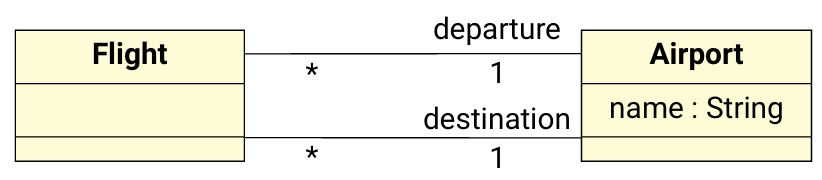
\includegraphics[width=1\textwidth]{Images/Example (Airport).jpeg}
\end{figure}

\subsection{Use of Associations in Domain Modelling}
\begin{defBox}[title=Heuristics]
    Include associations in the domain model when: \blue{Knowledge about the relation needs to be preserved for some time}
\end{defBox}
\begin{defBox}[title=Example]
    The relation between a \red{bill} and its \red{entries} needs to be remembered\\
    But it is unnecessary to store the relation between a customer and his or her most recent search for available cars\\
    On the other hand, a \red{browser} might well redcord the search history
\end{defBox}
List of common association \red{categories}:
\begin{itemize}
    \item A is a \red{transaction} related to another transacton B
    \item A is a \red{line item} of a transaction B
    \item A is a \red{product} or a \red{service} for a transaction B
    \item A is a \red{role} related to a transaction B
    \item A is a physical or logical \red{part} of B
\end{itemize}

\subsection{Association Name}
\begin{defBox}
    Name an association based on a \red{Class name-Verb phrase-Class name} format\\
    The verb phrase creates a sequence that is readable and meaningful
\end{defBox}
\blue{Good examples:}
\begin{itemize}
    \item Player \blue{Stands-on-} Square
    \item Sale-\blue{Paid-by}-CashPayment
\end{itemize}
\red{Bad examples:}
\begin{itemize}
    \item Player-\red{Has}-Square (\enquote{Has} is generic, doesn't tell about relation)
    \item Sale-\red{Uses}-CashPayment (\enquote{Uses} dito)
\end{itemize}

\subsection{Attribute or Association?}
\begin{defBox}
    A \red{property} can be modelled as an \red{association} or an \red{attribute}
\end{defBox}
\blue{The notations are very different! - When to use what?}
\begin{itemize}
    \item Attributes should always be used for \red{primitive} datatypes
    \begin{itemize}
        \item Boolean, Integer, Character, String
        \item Date, Address, Color, Phone Number, ...
    \end{itemize}
    \item Quantities \red{may} be modelled as classes to attach units
    \begin{itemize}
        \item currency (EUR, USD, SEK, ...)
        \item weight (kilogram, cm, ...)
    \end{itemize}
    \item \red{Always} use associations to model relations between conceptual classes
\end{itemize}
\begin{figure}[h]
    \centering
    \includegraphics[width=1\textwidth]{Images/Attribute or Association?.jpeg}
\end{figure}

\subsection{Refining a Model: Replace String Type}
\begin{defBox}
    It is convenient to type attributes \red{initially} with \blue{String}:\\
    \red{Generic} type that avoids \red{premature} decision\\
    Later, consider \red{refinement} to description class
\end{defBox}
\begin{figure}[h]
    \centering
    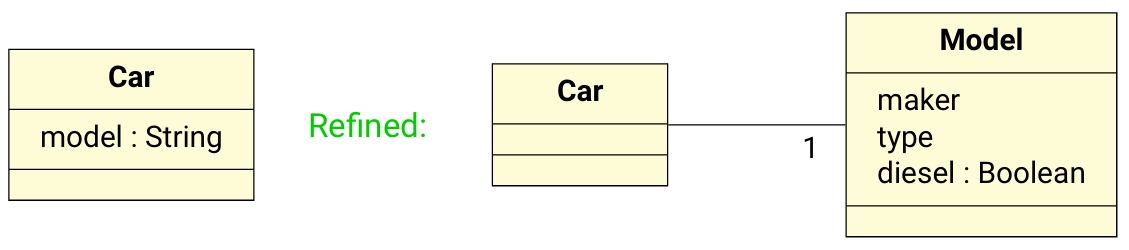
\includegraphics[width=1\textwidth]{Images/Refining a Model.jpeg}
\end{figure}
\begin{itemize}
    \item When string has \red{structure}, i.e. composed of separate sections: Maker, type
    \item When other \red{relations} are associated with the string: social security nr
    \item When the string has other \red{attributes}: diesel
    \item When the string is a quantity with a \red{unit}, for example, a currency
\end{itemize}

\subsection{CaSh Booking System: Domain Model (Excerpt)}
\begin{figure}[h]
    \centering
    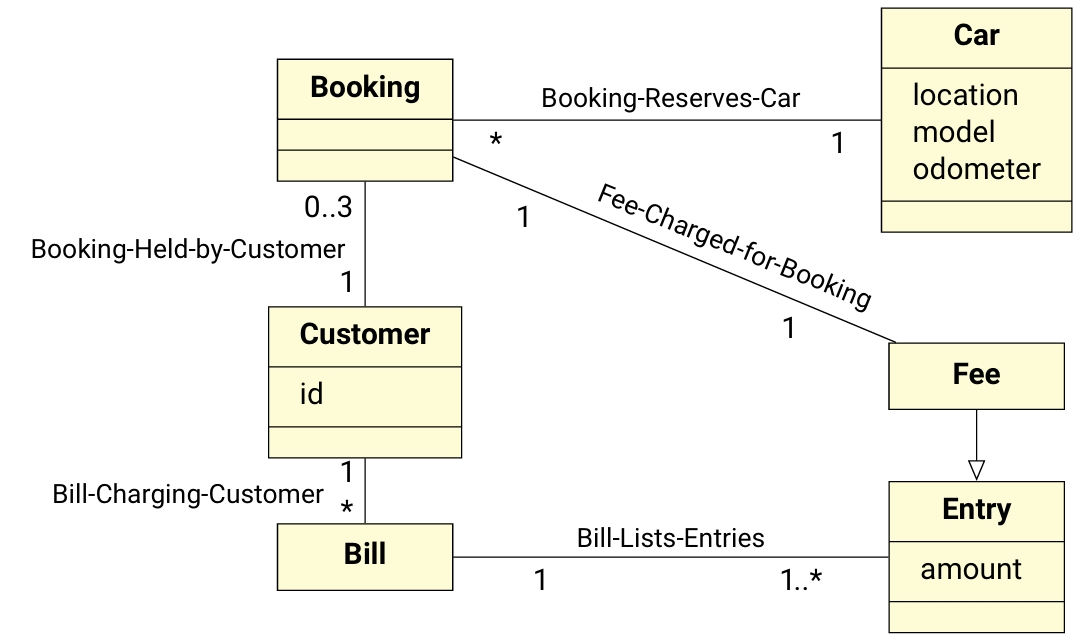
\includegraphics[width=1\textwidth]{Images/Domain Model (Excerpt).jpeg}
\end{figure}

\clearpage
\subsection{From Domain Model to Design model}
\begin{defBox}
    The domain model serves as a source of \red{inspiration} for the design model
\end{defBox}
\begin{figure}[h]
    \centering
    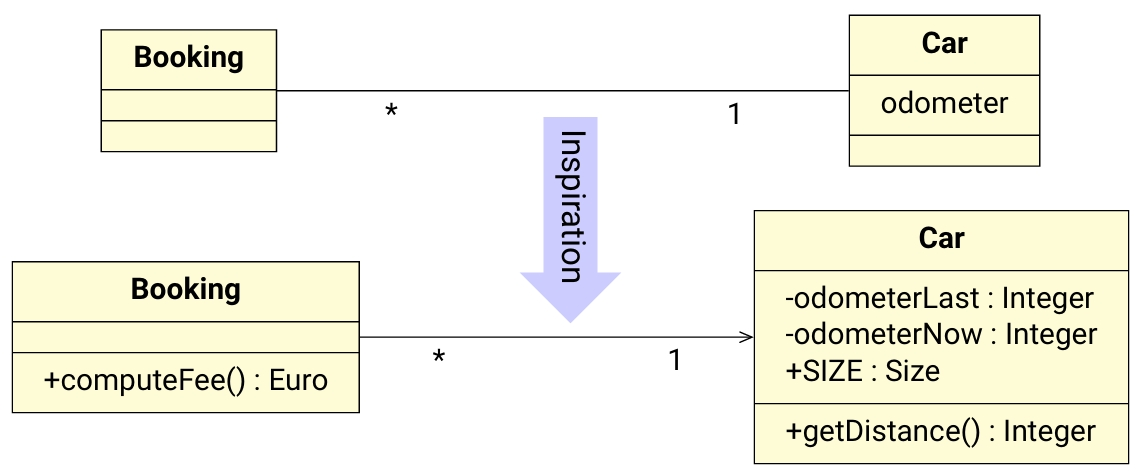
\includegraphics[width=1\textwidth]{Images/From Domain Model to Design Model.jpeg}
\end{figure}

\subsection{Domain Model is Not Static View on Code}
\begin{defBox}[title=The Two Faces of UML Class Diagrams]
    \begin{itemize}
        \item \red{Conceptual perspective model} in domain modelling (our usage)
        \item Static view (classes, methods, fields) extracted from \red{OO code}
    \end{itemize}
\end{defBox}
\begin{defBox}
    Don't confuse them, for example, abuse the former as code stubs
\end{defBox}

\section{Behavioral Models}
\subsection{Behavioral Domain Modelling}
\begin{defBox}
    Class diagrams model \red{static} aspects of software
\end{defBox}
\begin{itemize}
    \item Classes, objects
    \item Properties: attributes, associations
    \item Functions
\end{itemize}
\begin{defBox}
    What about \red{behavior}?
\end{defBox}
\begin{itemize}
    \item \red{Sequences of actions} and how they change the
    \begin{itemize}
        \item \red{state of a system}
        \item under which \red{condition}
    \end{itemize}
\end{itemize}

\subsection{UML State Machine Diagrams}
\begin{defBox}
    \red{UML State Machine Diagrams} are finite state machines whose transitions are equipped with \red{in-/output actions} and \red{guards}
\end{defBox}
\begin{figure}[h]
    \centering
    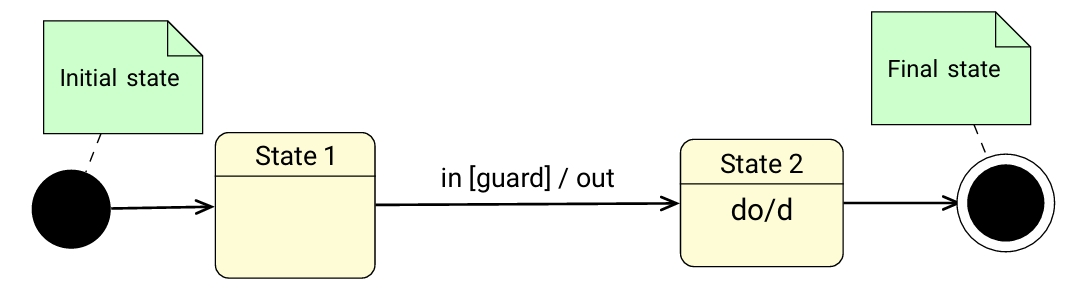
\includegraphics[width=1\textwidth]{Images/UML State Machine Diagrams.jpeg}
\end{figure}

\begin{defBox}[title=Semantics]
    When in \red{State 1}, if \red{input} in is observed and \red{guard} is true, then \red{output} out happens and current state becomes \red{State 2}.\\
    In \red{State 2} perform (interruptible) \red{action} d.
\end{defBox}

\subsection{Basic States}
\begin{figure}[h]
    \centering
    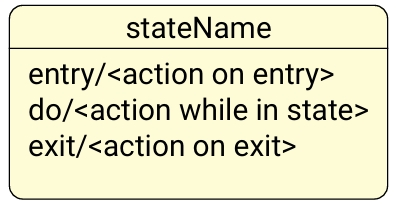
\includegraphics[width=0.5\textwidth]{Images/Basic States.jpeg}
\end{figure}
\begin{defBox}[title=Basic States in Detail]
    \begin{itemize}
        \item Basic states have a \red{name} and can define any combination of 
        \begin{itemize}
            \item \red{entry action:} action performed on state entry
            \item \red{do action:} action performed while in state (until the action terminates or the state is left)
            \item \red{exit action:} action performed on state exit
        \end{itemize}
        \item Actions are executed \red{operations}
    \end{itemize}
\end{defBox}

\clearpage
\subsection{Basic States: INitial, Final \& Terminal States}
\begin{figure}[h]
    \centering
    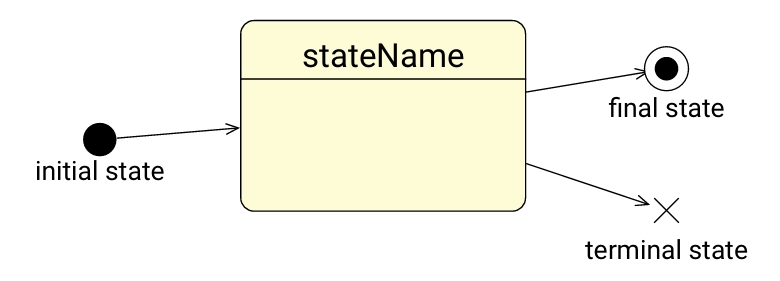
\includegraphics[width=0.5\textwidth]{Images/Initial, Final und Terminal States.jpeg}
\end{figure}
\begin{defBox}[title=States with Special Meaning]
    \begin{itemize}
        \item \red{Inital State:} has single transition to \red{first} entered state (may be labeled by object creation event/message)
        \item \red{Final State:} indicates completion of scenario
        \item \red{Terminal State:} completion and executing object destroyed
    \end{itemize}
\end{defBox}

\subsection{Transitions between States}
\begin{figure}[h]
    \centering
    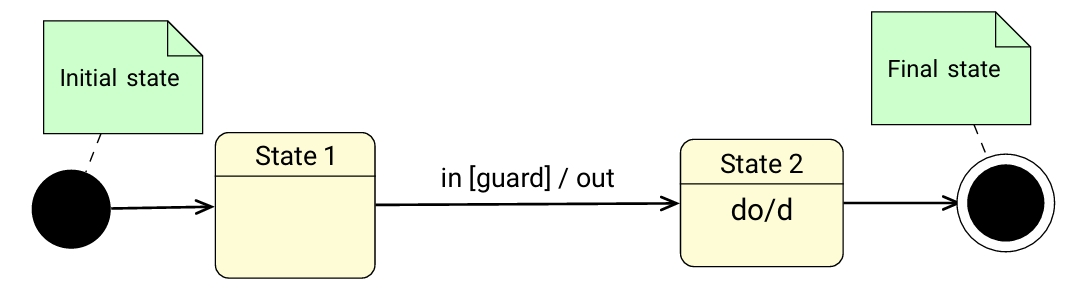
\includegraphics[width=1\textwidth]{Images/UML State Machine Diagrams.jpeg}
\end{figure}
\begin{defBox}[title=Transition Labels: input? ('[' guard ']')? '/' output?]
    \begin{itemize}
        \item All parts are optional (indicated by ?)
        \item \red{Input} (trigger) events are observations such as:
        \begin{itemize}
            \item call event (start of operation)
            \item time event (for example, time spent in a state)
            \item change event (value of an attribute has changed)
        \end{itemize}
        \item \red{gaurd} is a Boolean expression
        \item \red{Output} (action) is an operation or domain-specific action expression
    \end{itemize}
\end{defBox}

\clearpage
\subsection{State Machine Diagram: Example (Credit Card Payment with PIN)}
\begin{figure}[h]
    \centering
    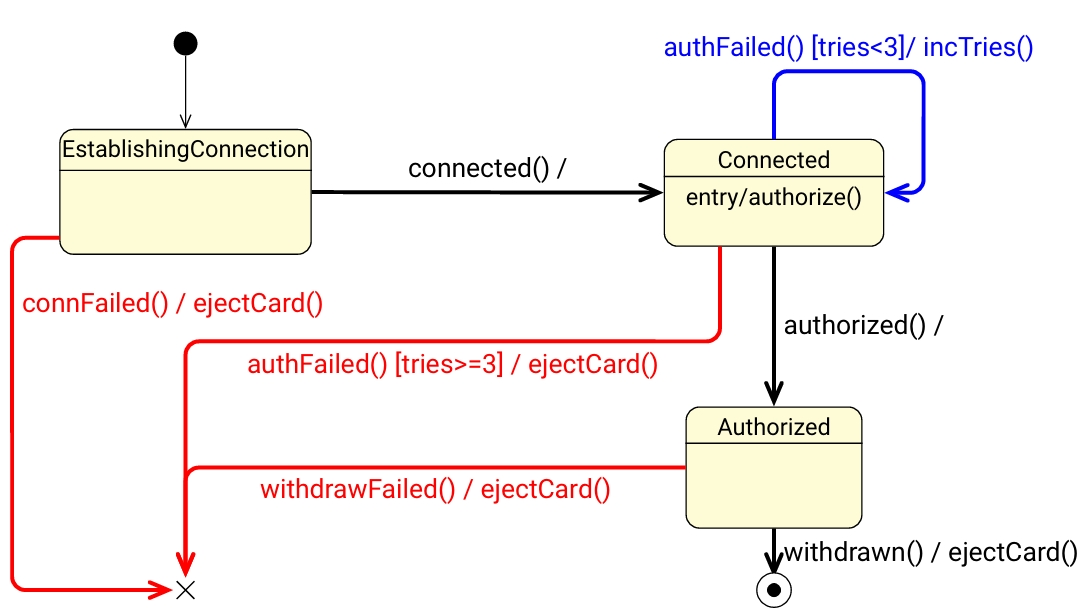
\includegraphics[width=1\textwidth]{Images/State Machine Diagram.jpeg}
\end{figure}

\subsection{State Machine Diagrams in Domain Modelling}
\begin{defBox}
    During domain modelling: State machine diagrams \red{do not relate to code}
\end{defBox}
\begin{defBox}[title=Uses of State Machine Diagrams in Doamin Modelling]
    \begin{itemize}
        \item Capture the action sequence of a \red{use case}
        \item \red{Combine} several, related use cases
        \item Clarify the \red{states} an object can be in
        \item Help to clarify \red{protocols}
        \item Help to \red{validate} the domain model
        \item Help to \red{complete} the domain model (with properties / actions)
    \end{itemize}
    State machine diagrams should only be used to model \red{non-trivial behavior}
\end{defBox}